\documentclass[a4paper,12pt]{article} 


\usepackage[T2A]{fontenc}			% кодировка
\usepackage[utf8]{inputenc}			% кодировка исходного текста
\usepackage[english,russian]{babel}	% локализация и переносы


% Математика
\usepackage{amsmath,amsfonts,amssymb,amsthm,mathtools} 

\usepackage{gensymb}	
\usepackage{wasysym}

% Картинки
\usepackage{graphicx}
\graphicspath{{images/}}

%Заговолок
\usepackage[left=2cm,right=2cm,
    top=2cm,bottom=2cm,bindingoffset=0cm]{geometry}

\usepackage{titling}


\author{Петров Артём Антонович, группа 721}
\title{Лабораторная работа № 3.4.2 "Закон Кюри-Вейеса (Температура Кюри)"}
\date{\today}

\begin{document} % начало документа

\begin{minipage}[t][5cm]{\textwidth}
\maketitle
\end{minipage}

%
%\textbf{Цель работы:} 
%\bigskip
%
%\medskip
%\textbf{Оборудование:} 
%\bigskip
%
%\subsection*{Теоретическое введение}
%\bigskip


\bigskip

\subsection*{Экспериментальная установка}
\bigskip


\begin{figure}[ht]
\centering
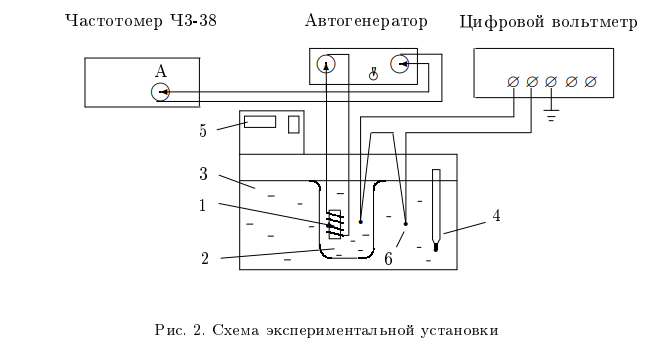
\includegraphics[width=160mm]{scheme.png}
\caption{Схема установки: 1 - образец из гадолиния, 2 - ёмкость с маслом, 3 - термостат ( объём с водой) и 5 - его управляющий блок, 4 - термометр (соединён с термостатом), 6 - термопара (для оценки процессов установления теплового равновесия). Период колебаний автогенератора без образца $t_0 = 6,9092\mu s$, коэф. термопары $k=24 \degree C/mV$.}
\label{schema}
\end{figure}

\bigskip

\subsection*{Ход работы}
\bigskip

Была получена зависимость периода колебаний автогенератора от температуры в термостате и показаний термопары (таблица \ref{table1}).

\begin{figure}[ht!]
\centering
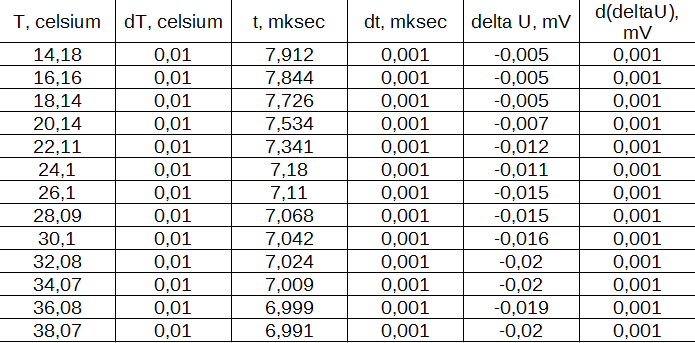
\includegraphics[width=160mm]{table1.png}
\caption{Зависимость периода от температура, полученная при измерениях.}
\label{table1}
\end{figure}

По этой зависимости была рассчитана зависимость величины обратной разности квадратов периодов колебаний с присутствием образца гадолиния и без него $1/(t^2-t_0^2)$ (эта величина пропорциональна $1/\chi$) от температуры $T$ (таблица \ref{table2}, график \ref{graph1}).

\begin{figure}[ht!]
\centering
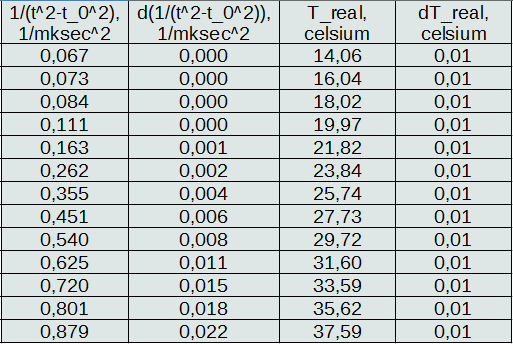
\includegraphics[width=160mm]{table2.png}
\caption{Зависимость величины обратной разности квадратов периодов колебаний с присутствием образца гадолиния и без него $1/(t^2-t_0^2)$ от температуры $T_{real}$, полученной с учётом показаний термопары.}
\label{table2}
\end{figure}

\begin{figure}[ht!]
\centering
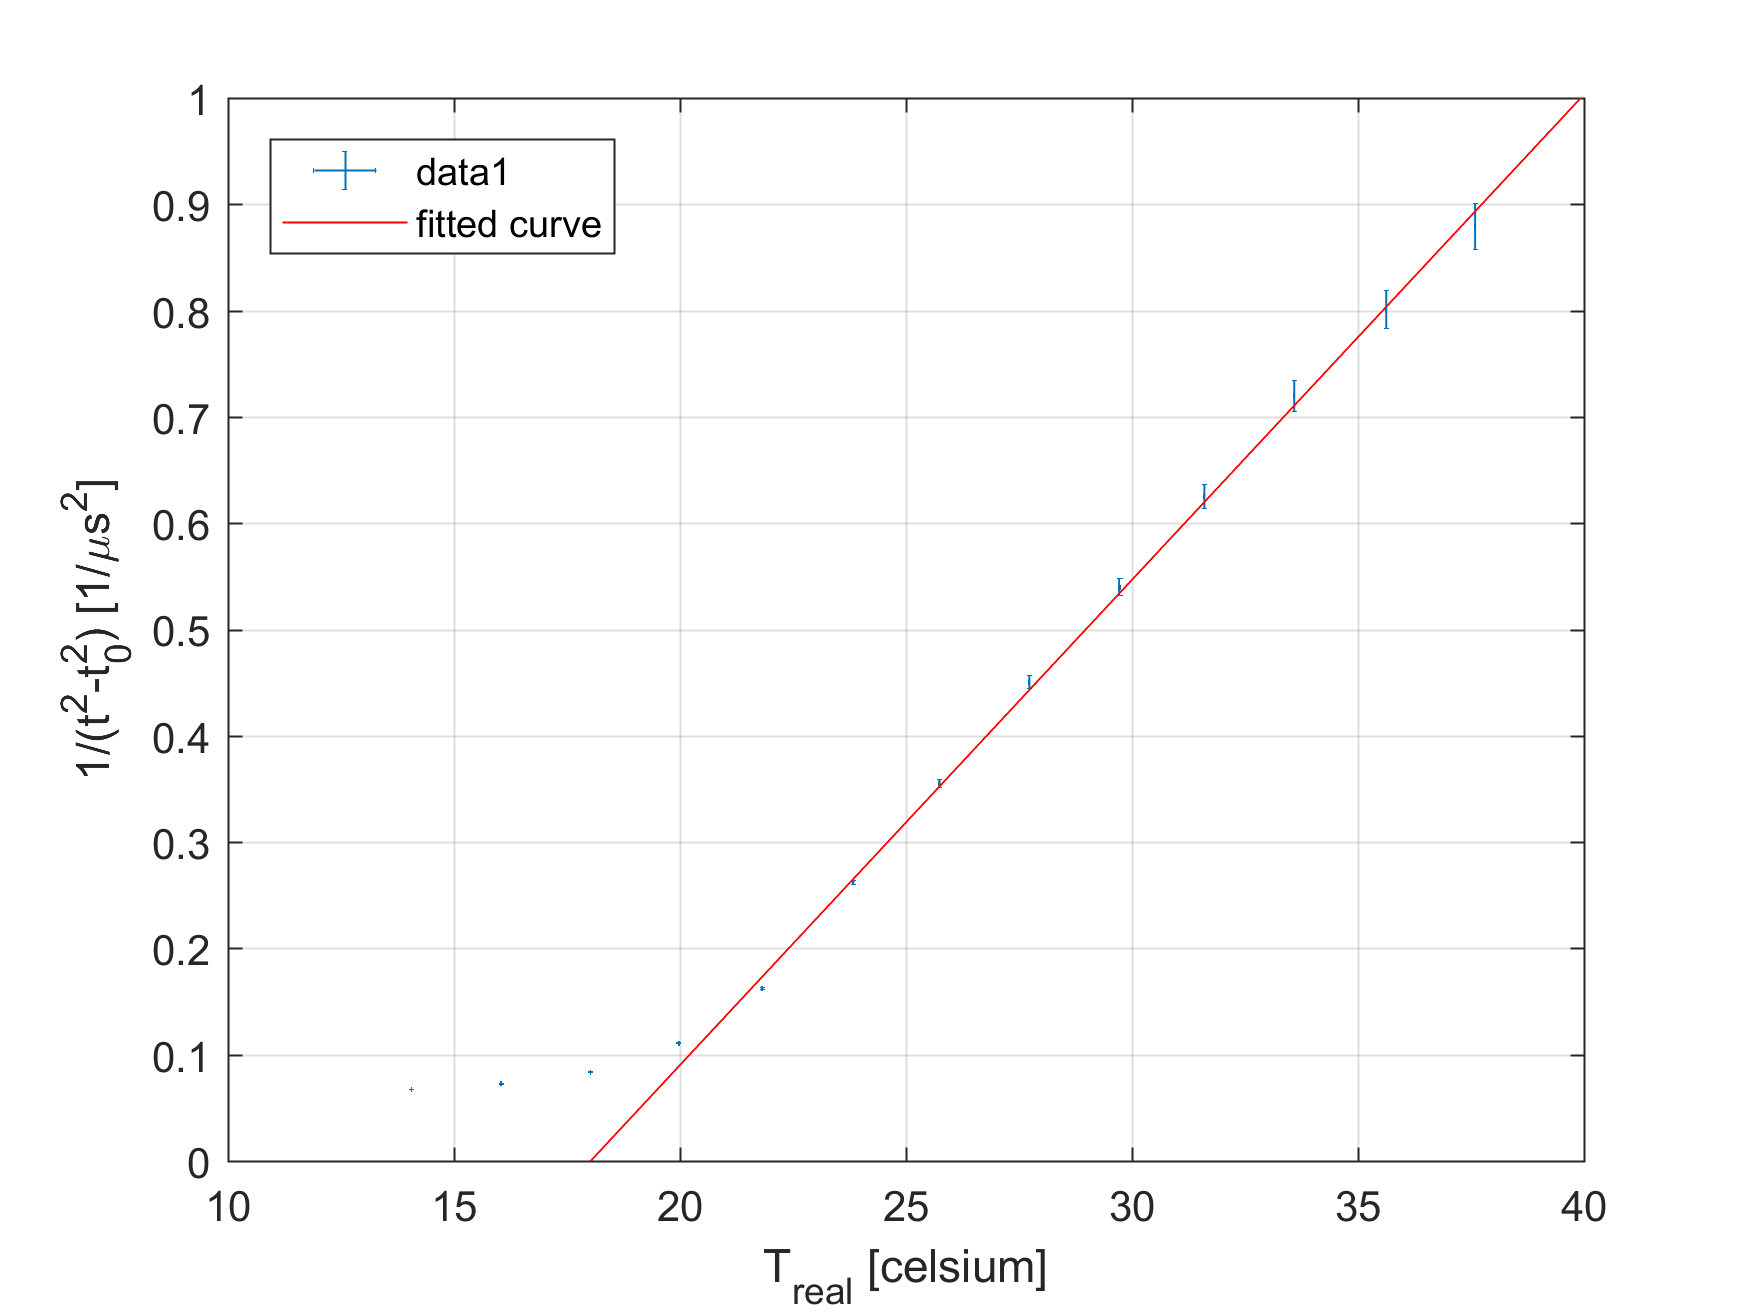
\includegraphics[width=160mm]{Plot1.png}
\caption{Зависимость величины обратной разности квадратов периодов колебаний с присутствием образца гадолиния и без него $1/(t^2-t_0^2)$ от температуры $T_{real}$, полученной с учётом показаний термопары.}
\label{graph1}
\end{figure}

С помощью экстраполяции было получено значение $\theta_p = 18,0 \pm 0,4 \degree C$.(из теории известно, что этот график пропорционален зависимости $1/\chi(T)$ и точка его пересечения с осью абсцисс есть $\theta_p$)

\bigskip
\subsection*{Итог}
\bigskip
 
 С помощью экстраполяции полученных данных было получено значение $\theta_p = 18,0 \pm 0,4 \degree C$, что совпадает с табличным значением $19 \degree C$. А также форма полученного графика совпадает с теоритическими предсказаниями, а значит закон Кюри-Вейеса выполняется.
 
\end{document} % конец документа